
\chapter{相关技术}

本章系统阐述了云边协同、云原生、模型部署及Actor编程模式的背景知识。首先,从基本概念出发,详细解析了云边协同的“端-边-云”三层架构,并进一步探讨了其垂直与水平方向的优化策略;随后,围绕云原生技术体系,依次介绍了容器化技术、Kubernetes集群管理及系统监控方案,为云边协同的分布式实现构建了技术基础;接着,重点阐述了模型部署的关键技术路径;最后,针对分布式系统需求,深入介绍了基于Actor模型的Akka框架设计原理。

\section{云边协同计算架构}

云边协同是在云计算和边缘计算两种典型计算范式的基础上发展起来的,旨在充分发挥两者的优势,以实现低延迟、高可用的数据处理\cite{李波2021基于软件定义网络的云边协同架构研究综述}。在传统的云边协同架构中,当请求在终端设备上产生时,轻量级请求通常可以直接由设备本地处理,而较复杂的请求则需要分发到附近的边缘服务器进行处理。边缘服务器处理完成后,结果会立即返回终端设备,从而保证较低的响应延迟。然而,边缘服务器的计算和存储能力有限,通常只能支持有限的应用和功能,因此对于无法快速处理的请求,最终将被转发到云计算中心进行处理。云边协同的架构通常可以分为“端-边-云”三个层级\cite{mao2017survey,satyanarayanan2017emergence,吴大鹏2018端},如图 \ref{fig:2-1云边端架构} 所示。

\begin{itemize} 
    \item \textbf{端层(End Layer)}:位于网络的最前端,包括物联网设备、传感器及终端用户设备。端层负责直接与现实世界交互,进行数据采集和初步处理,如数据过滤或简单分析。同时,端层设备通过无线或有线连接与边层节点进行数据传输和指令通信,确保信息的及时传递与响应。
    \item \textbf{边层(Edge Layer)}:由边缘服务器、网关及边缘计算节点等设备组成,处于端层与云层之间。边层节点靠近数据源,具备一定计算和存储能力,能够对来自端层的数据进行实时处理与分析,执行较为复杂的计算任务,并在必要时与云层节点进行通信,以协调更大规模的资源和服务。
    \item \textbf{云层(Cloud Layer)}:通常由大型云计算数据中心构成,提供强大的计算、存储和网络资源。云层节点负责处理需要大规模计算能力的任务,进行深度数据分析和机器学习模型训练,并管理和存储海量数据。云层还支持跨地域的资源调度和服务集成,提供全局性的决策支持和业务逻辑。
\end{itemize}

\begin{figure}[ht]
  \centering
  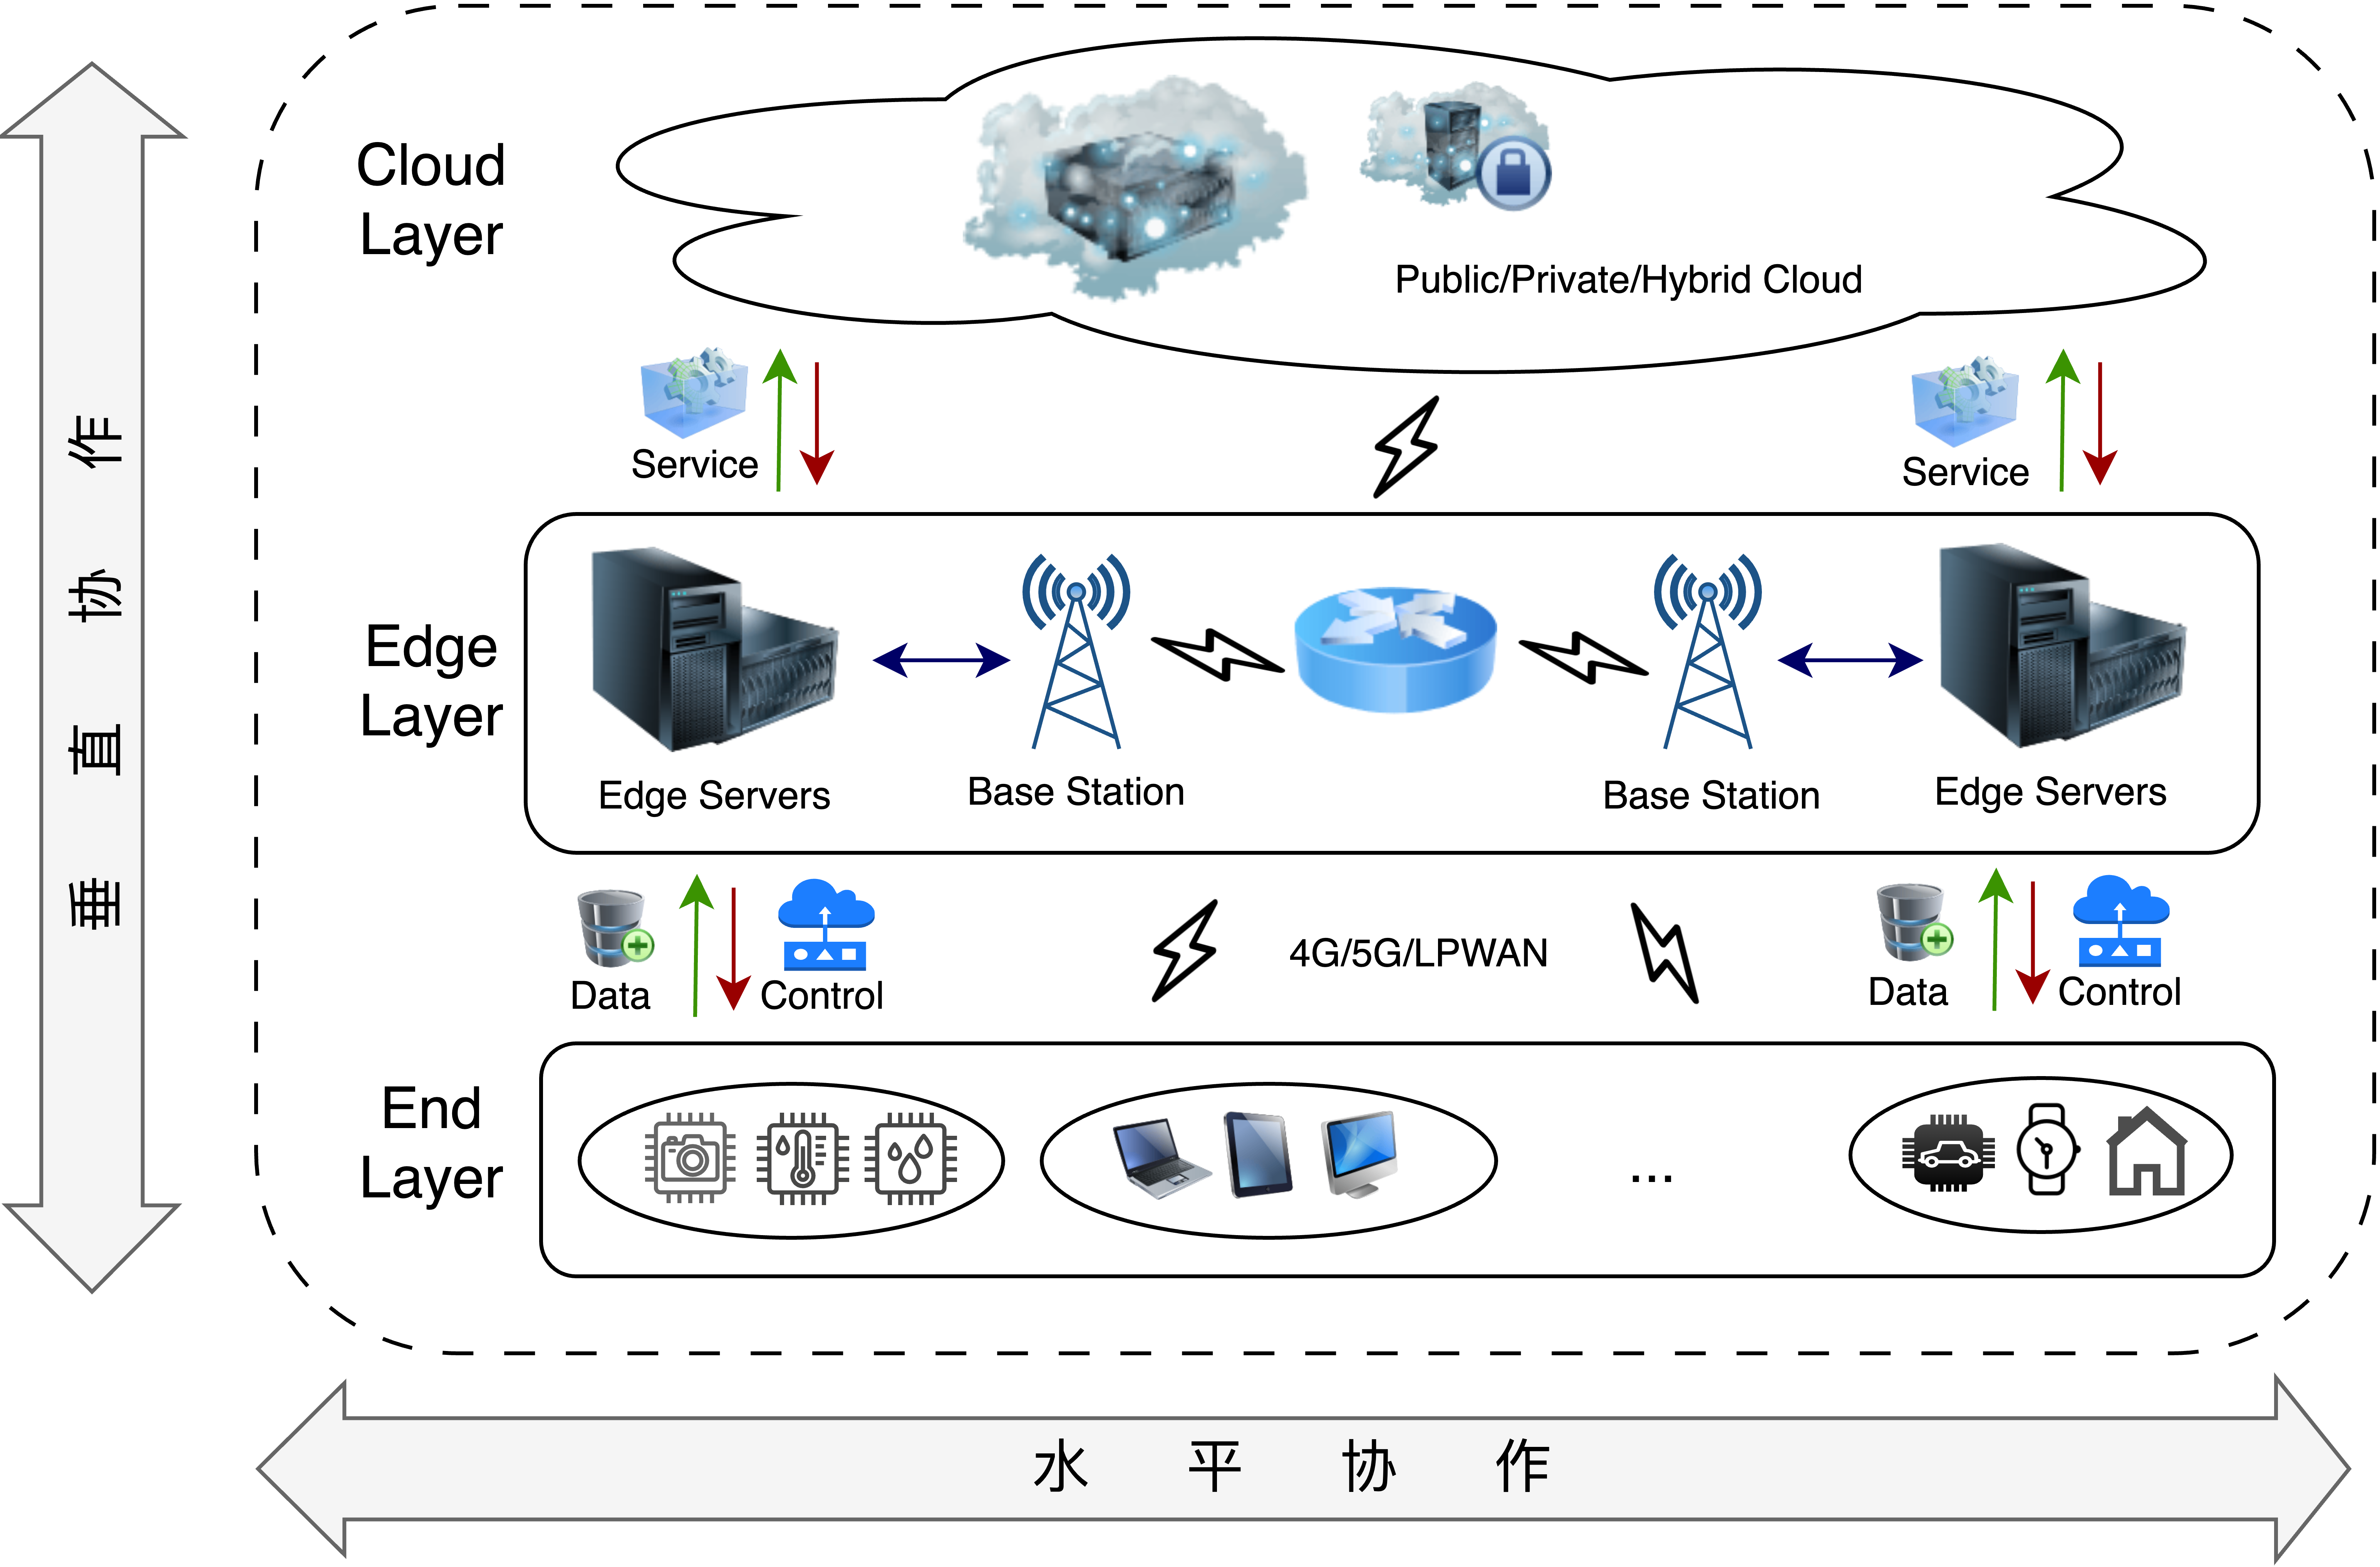
\includegraphics[width=\linewidth]{pics/2-1云边端架构.png}
  \caption{云边协同的“端-边-云”三层架构\cite{mao2017survey,satyanarayanan2017emergence,吴大鹏2018端}}
  \label{fig:2-1云边端架构}
\end{figure}

部分研究\cite{lane2016deepx,teerapittayanon2017distributed,liu2023adaptive}进一步指出,具有初步计算能力的端层设备也可与边缘服务器协同完成推理任务。为便于论述,本研究将这类端层设备与边层节点统一视为“边”,而将云层节点称为“云”。通过这种分层架构,云边协同能够有效利用不同层级的计算资源,从垂直和水平两个角度进行资源优化\cite{dupont2017edge,li2020elastic}。垂直优化指的是在“端-边-云”各层之间进行资源分配与优化,需要将云端和边缘端的硬件资源进行虚拟化抽象,并依据应用需求统一管理与分配。基于应用特性,计算任务可以被合理地部署在云端或边缘端,同时在层次之间需优化传输路径协议,并采取加密等手段保障数据安全。水平优化则关注同一层级内的资源协同,特别是边缘节点之间的协作计算。通过任务分割和并行计算,水平优化能够提升计算效率。通过动态监测边缘节点的负载情况,系统能够将计算任务合理分配到负载较轻的节点,进而利用负载均衡算法优化资源的使用,提升整体计算性能。

\section{云原生技术}

\subsection{容器化技术}

容器化技术作为一种轻量级的虚拟化方法,通过将应用程序及其依赖项封装到独立的运行环境中,有效解决了底层硬件架构和操作系统的异构性问题。如图\ref{fig:2-2container}所示,容器化架构通过标准化的运行时接口与镜像格式,构建了跨平台部署的统一抽象层,从而显著提升了应用的可移植性和部署效率。在边缘计算场景中,这一特性尤为重要。由于边缘设备通常涉及多种硬件架构(如x86、ARM)以及多样化操作系统(如Linux、Windows),容器化技术通过提供一致的运行时环境和标准化的镜像分发机制,不仅简化了跨平台应用的开发与部署流程,还为动态迁移和资源调度提供了可靠的技术保障\cite{urblik2024containerization}。

\begin{figure}[ht]
  \centering
  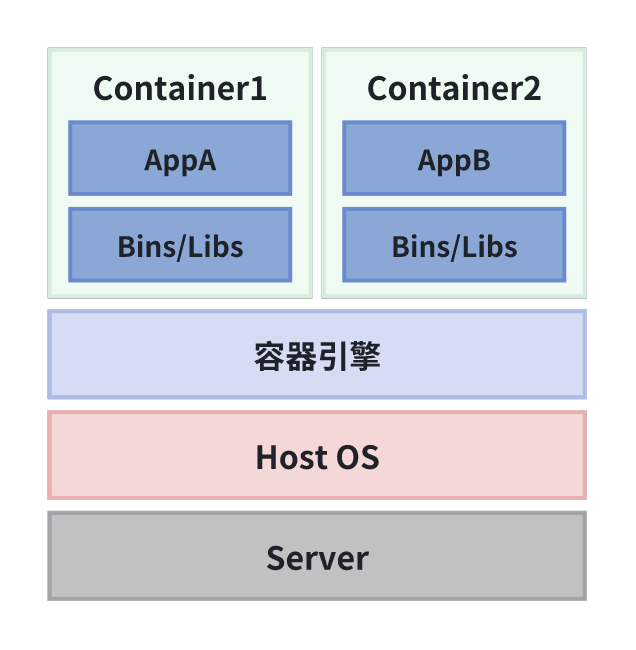
\includegraphics[width=0.5\linewidth]{pics/2-2container.png}
  \caption{容器化技术架构\cite{urblik2024containerization}}
  \label{fig:2-2container}
\end{figure}

目前,常见的容器化技术包括 Docker 和 containerd。Docker 通过分层文件系统实现高效的镜像管理,并提供用户友好的命令行工具和丰富的生态系统,显著降低了容器技术的使用门槛。而 containerd 是一个轻量级的容器运行时,专注于容器生命周期管理,具有高性能和低资源开销的特点,适合大规模生产环境。

\subsection{Kubernetes}

Kubernetes 是由 Google 发起并开源的容器编排系统,目前由 CNCF(Cloud Native Computing Foundation)维护。作为云原生技术的核心组件,Kubernetes 提供了一套完整的解决方案,用于自动化容器化应用的部署、扩展与管理。其核心功能涵盖服务发现与负载均衡、存储编排以及密钥和配置管理等。此外,Kubernetes 借助声明式 API 实现了系统状态的自动收敛,开发者只需定义期望的状态,Kubernetes 便会自动调整实际状态以匹配期望值,从而为云原生应用提供了可扩展的部署框架。

\begin{figure}[ht]
  \centering
  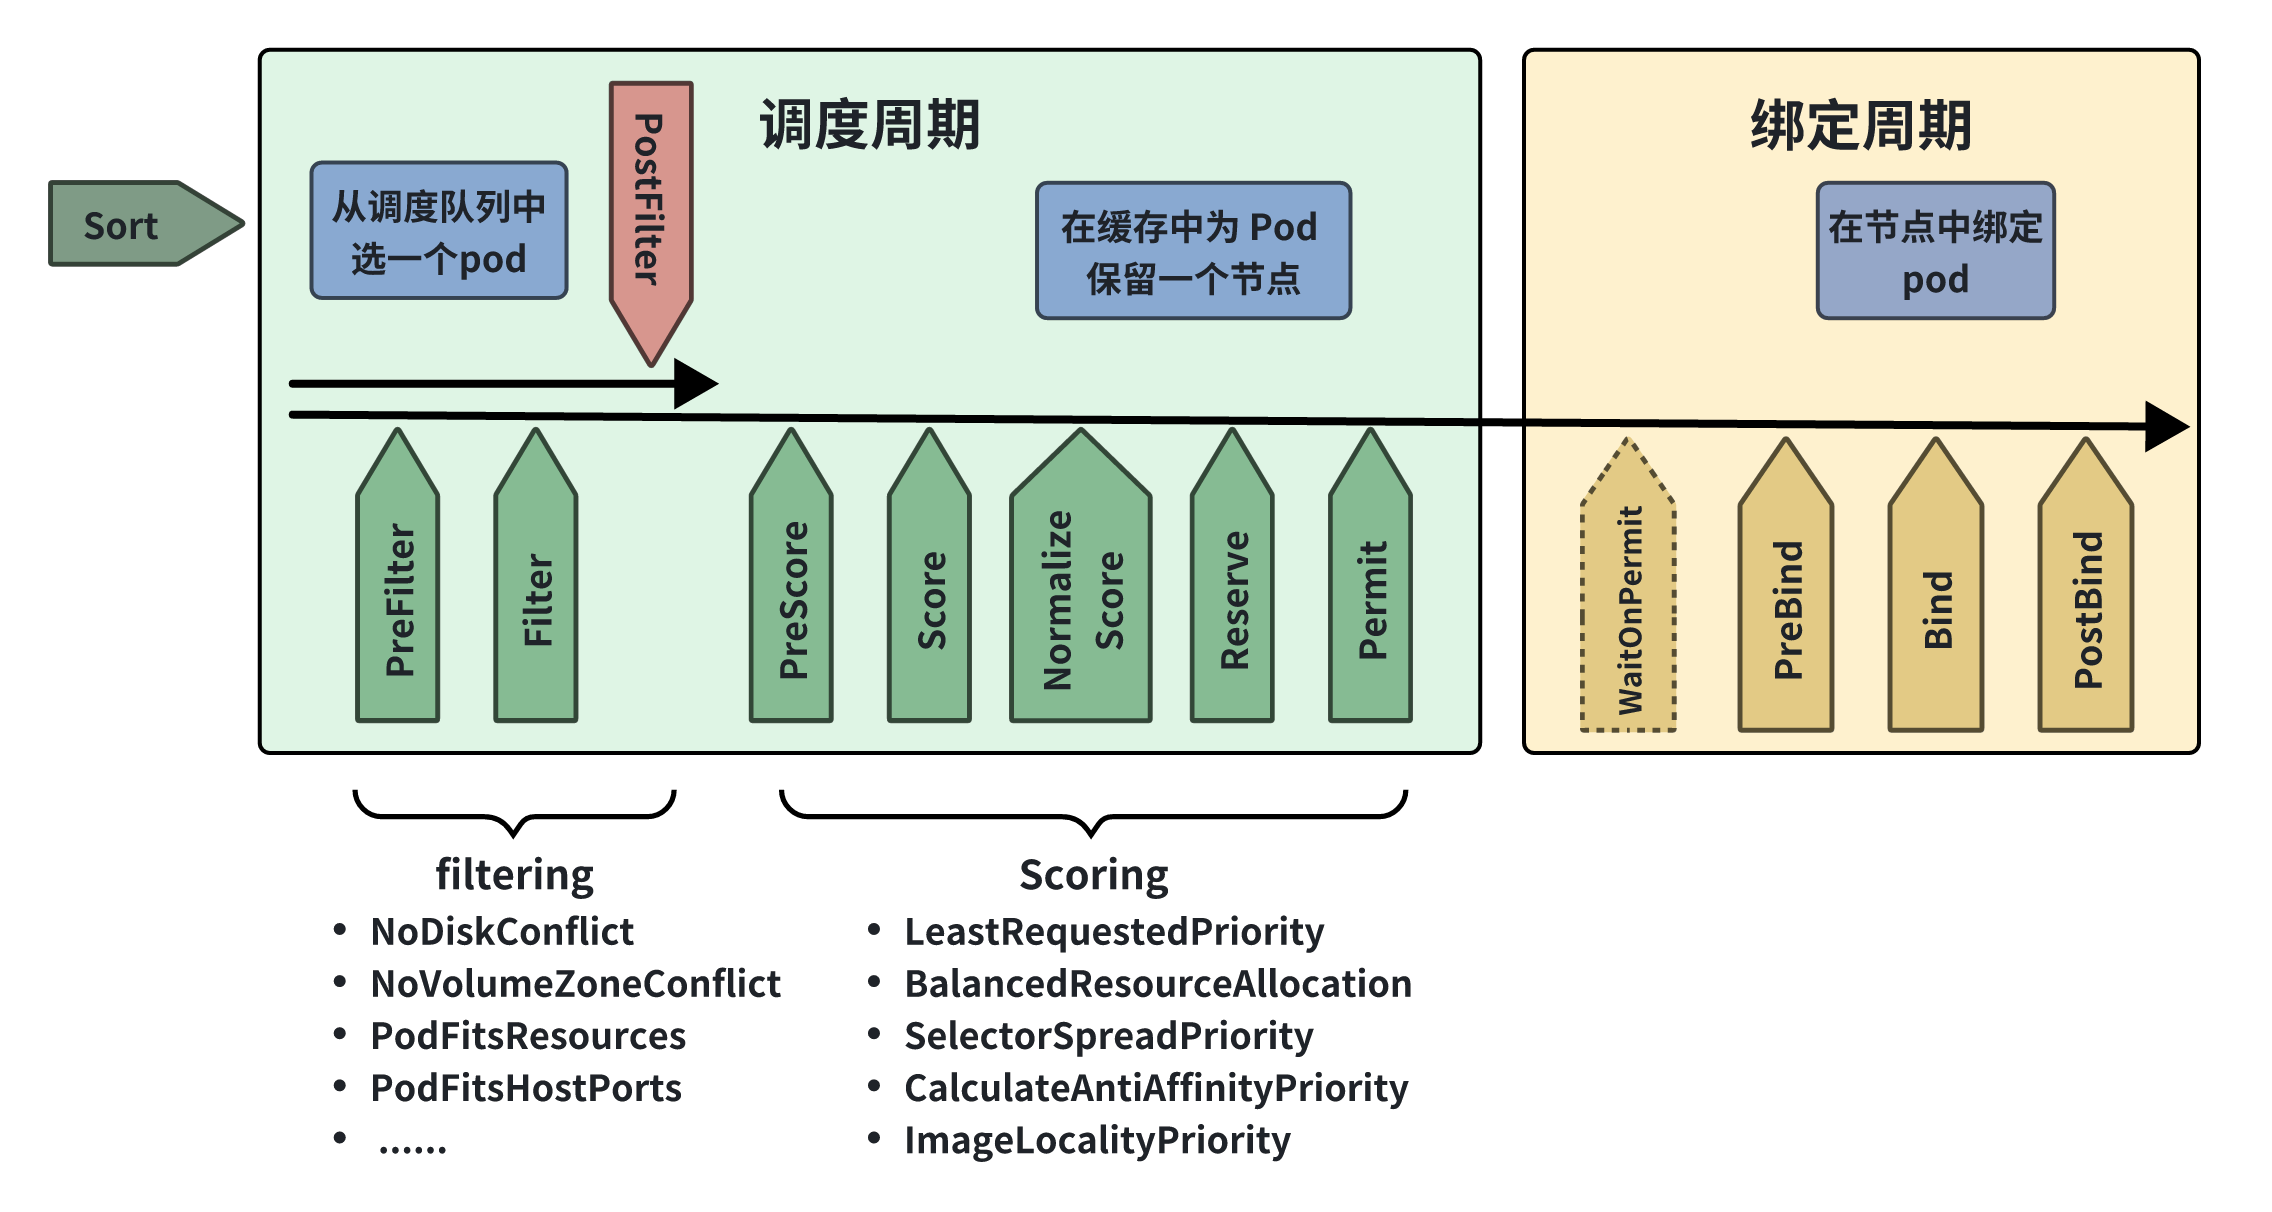
\includegraphics[width=\linewidth]{pics/2-4k8sschedule.png}
  \caption{Kubernetes 中的负载调度方案\cite{kubernetes}}
  \label{fig:2-4k8sschedule}
\end{figure}

在 Kubernetes 的众多功能中,资源调度是其核心能力之一。如图 \ref{fig:2-4k8sschedule} 所示,Kubernetes 调度器采用两阶段决策模型实现资源分配。首先,在过滤(Filtering)阶段,调度器根据资源需求、亲和性规则、反亲和性规则等条件,排除不符合要求的节点,生成可行节点列表。接着,在打分(Scoring)阶段,调度器结合资源平衡、数据本地性等因素对可行节点进行评分,并选择得分最高的节点作为目标节点。如果存在多个得分相同的节点,则随机选择其中一个进行绑定。通过这种机制,Kubernetes 能够综合考虑节点的硬件性能、网络拓扑结构以及存储类型等特性,合理分配任务,从而有效优化资源利用率并提升应用性能。

\subsection{系统监控技术}

\subsubsection{通信监控}

边端节点通常分布在异构网络环境中,其通信性能容易受到网络带宽、延迟、丢包率以及通信协议开销等多种因素的影响。为了解决这一问题,Haja 等人\cite{haja2019sharpening} 提出了一种实时监测边缘节点间传输时延的方法。该方法在每个节点上部署测量 Pod,这些 Pod 定期发送 ping 包并记录往返时间,从而生成延迟数据,如图 \ref{fig:2-6ping} 所示。此设计能够提供实时的通信性能评估,为动态优化和调度策略的制定提供数据支持。

\begin{figure}[ht]
  \centering
  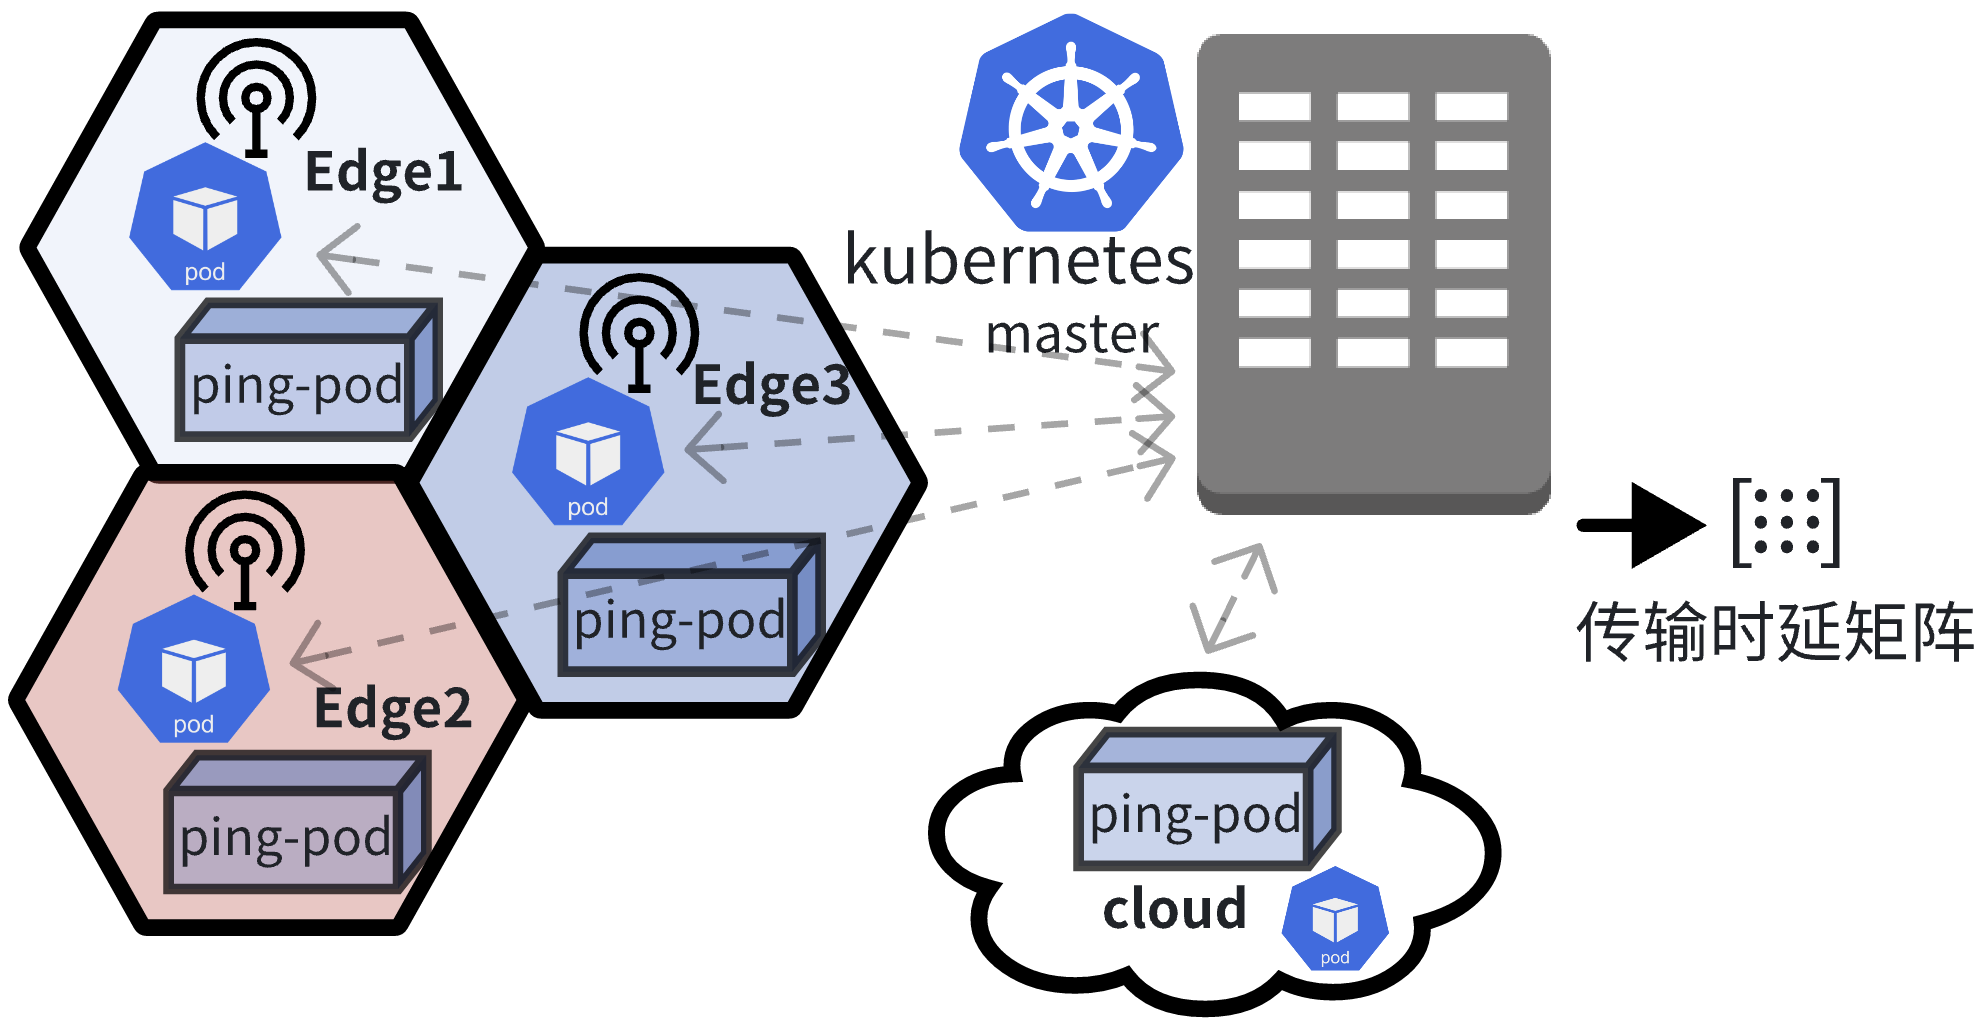
\includegraphics[width=0.75\linewidth]{pics/2-6ping.png}
  \caption{基于Ping的传输时延监测\cite{haja2019sharpening}}
  \label{fig:2-6ping}
\end{figure}

在节点间通信监测中,Ping 和 iperf3 是常用的技术方案,各有其特点和适用场景。Ping 是一种轻量级工具,通过发送 ICMP 请求快速检测网络连通性和往返延迟(RTT),适用于实时性要求高的基础连通性监测。然而,Ping 功能较为单一,无法提供带宽等深入的性能数据。相比之下,iperf3 提供更详尽的网络性能指标,包括带宽、抖动和丢包率,支持 TCP 和 UDP 协议,适合需要深入分析网络质量的场景。不过,iperf3 的部署较为复杂,且因其占用较多网络资源,不适合实时或生产环境的持续监测。

\subsubsection{模型推理性能监测}

边缘节点具有显著的异构性,其硬件资源配置多样化,包括低功耗CPU、多核GPU以及专用AI加速器(如VPU)等。这种硬件异构性导致节点在计算能力、存储容量和能耗限制上存在显著差异,从而增加了资源分配与利用优化的复杂性。

\begin{figure}[ht]
  \centering
  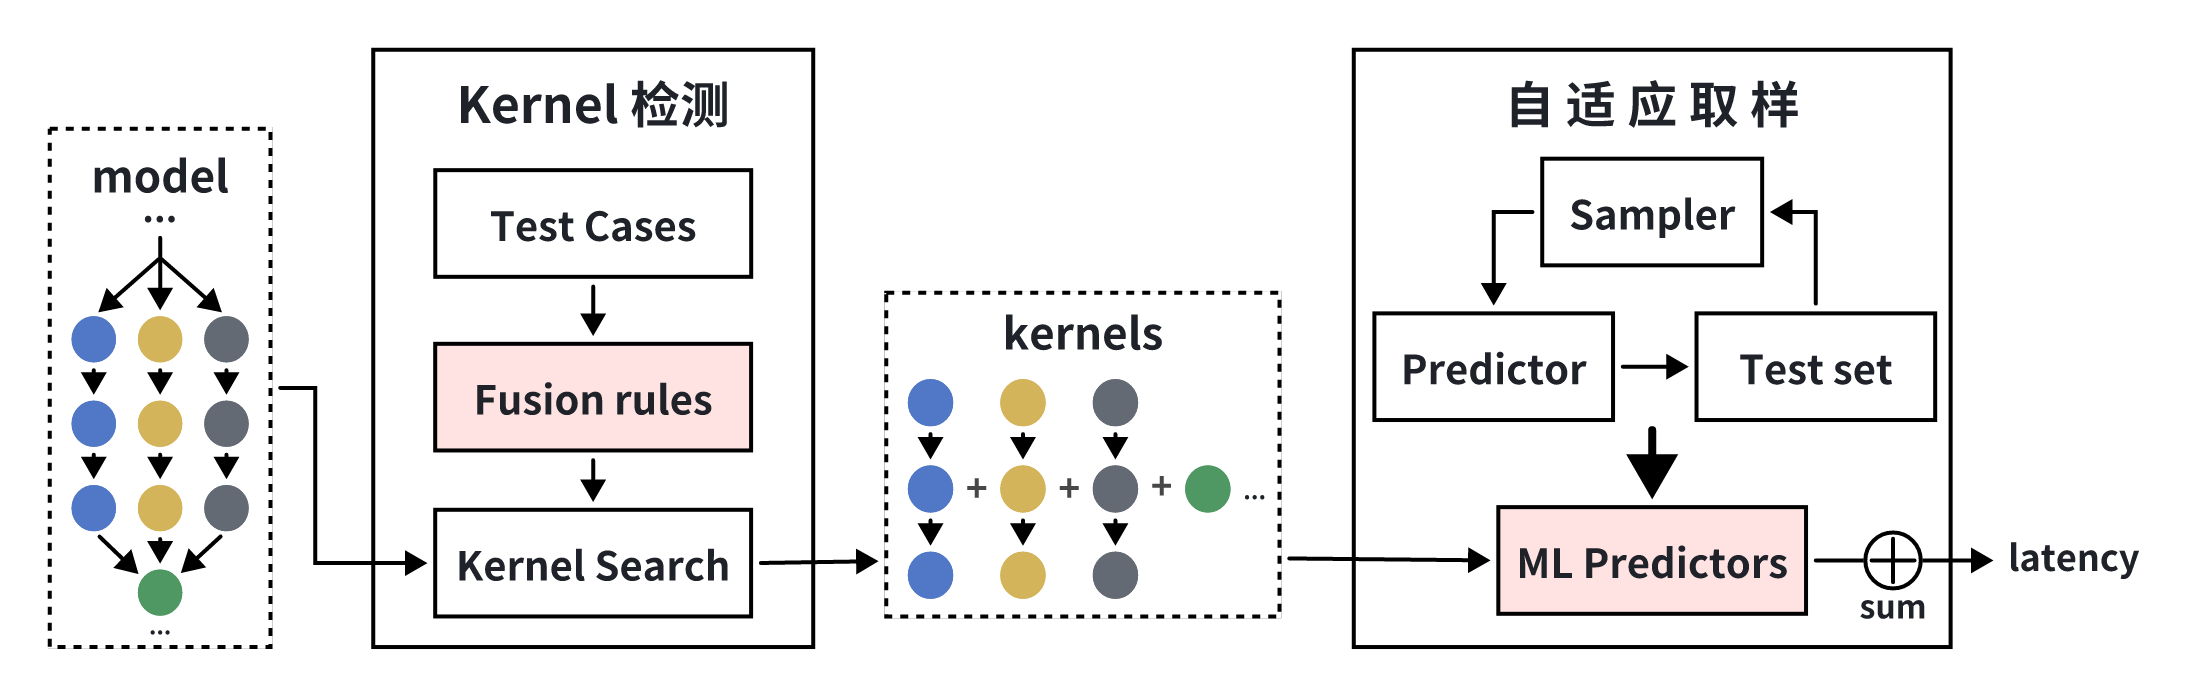
\includegraphics[width=\linewidth]{pics/2-5nnmeter.png}
  \caption{nn-Meter工具的架构\cite{zhang2021nn}}
  \label{fig:2-5nnmeter}
\end{figure}

在边端评估深度学习模型推理性能时,推理时延是一个关键指标。部分学者\cite{he2018amc,tan2019mnasnet}提出了基于浮点运算次数(FLOPs)的方法。该方法通过估算模型的FLOPs快速预测推理时延,无需实际部署模型,适用于初步筛选阶段。然而,FLOPs仅从理论层面反映计算复杂度,无法充分考虑硬件特性,因此其预测结果与实际时延可能存在显著偏差,仅适用于精度要求较低的场景。为解决上述问题,Zhang 等人\cite{zhang2021nn} 提出了 nn-Meter 工具,旨在更准确地预测不同边缘设备上的模型推理时延。nn-Meter 的核心思想是通过设计测试用例,自动检测模型在特定设备上的推理执行单元(即内核)及算子融合规则,并递归地将模型划分为多个内核,从而精确捕获设备的实际执行行为。如图 \ref{fig:2-5nnmeter} 所示,nn-Meter 的关键技术包括:首先,根据模型结构和硬件延迟特性对内核配置进行剪枝;其次,通过迭代采样选择最优配置进行检测,而非随机选择;最后,利用机器学习回归器学习采样数据的非线性关系,构建高效的内核级延迟预测器。实验表明,这种方法显著提高了时延预测的准确性。然而,nn-Meter 目前尚无法支持对模型在批处理情况下的性能测试,这为其进一步应用带来了一定限制。

\subsubsection{Promethus}

Prometheus 是云原生领域中被广泛采用的核心监控系统,其设计目标是为动态化、分布式的云环境提供高效、灵活且可靠的监控解决方案。作为 CNCF 的毕业项目,Prometheus 的核心功能在于通过其高性能的时间序列数据库采集、存储和查询多维监控数据,同时支持用户根据需求配置灵活的告警规则。它采用了 拉取(Pull)模式的工作机制,这意味着 Prometheus Server 会主动从目标系统中定期拉取指标数据,而不是依赖目标系统主动推送数据。这种设计不仅简化了架构复杂性,还提升了系统的可控性和稳定性。为了实现对监控数据的精细化管理,Prometheus 引入了带有标签(Labels)的时间序列模型,通过标签对时间序列进行标识与分类,从而支持细粒度的数据筛选、聚合和分析能力。

在 Prometheus 的生态系统中,多个核心组件协同工作以完成完整的监控闭环。Prometheus Server 是整个系统的核心,负责数据的采集、存储以及查询处理;Exporters 则扮演了数据适配器的角色,用于将不同目标系统的内部指标暴露为 Prometheus 可识别的标准格式,例如 Node Exporter 用于采集主机级别的指标,而 Blackbox Exporter 则专注于网络探测和黑盒测试;Alertmanager 是 Prometheus 告警管理的关键组件,能够对告警信息进行去重、分组和路由,并通过邮件等多种渠道发送通知,确保告警信息能够及时送达相关人员;PromQL(Prometheus Query Language)作为一种专为时间序列数据分析设计的查询语言,提供了强大的表达能力和灵活性,使用户能够对复杂的监控场景进行深度挖掘和精准定位。此外,Grafana 作为与 Prometheus 深度集成的开源可视化平台,可将时序数据转化为直观的图表与仪表盘,助力系统状态监控与性能趋势分析。

\section{模型部署相关技术}

在AI模型从开发到生产部署的全生命周期中,跨框架兼容性与高效推理服务是两大核心挑战。在模型标准化方面,ONNX(Open Neural Network Exchange)\cite{bai2017onnx} 提供了一种开放的跨框架模型交换格式,旨在增强模型在不同开发环境中的兼容性与灵活性。通过将模型转换为统一的中间表示(Intermediate Representation, IR),ONNX 实现了模型在多种主流深度学习框架(如 TensorFlow、PyTorch、MXNet 等)之间的无缝迁移。如图 \ref{fig:2-6onnx} 所示,ONNX 的工作流程通常包括两个阶段:首先,原始模型被导出为 ONNX 格式的中间状态;然后,该中间状态可以进一步转换为目标框架支持的格式。这一过程不仅减少了模型迁移的技术壁垒,还支持通过模型驱动的方式优化推理性能。此外,ONNX 提供了丰富的算子库和工具链(如 ONNX Runtime),使得开发者能够在不改变模型结构的前提下实现高效的推理加速。

\begin{figure}[ht]
  \centering
  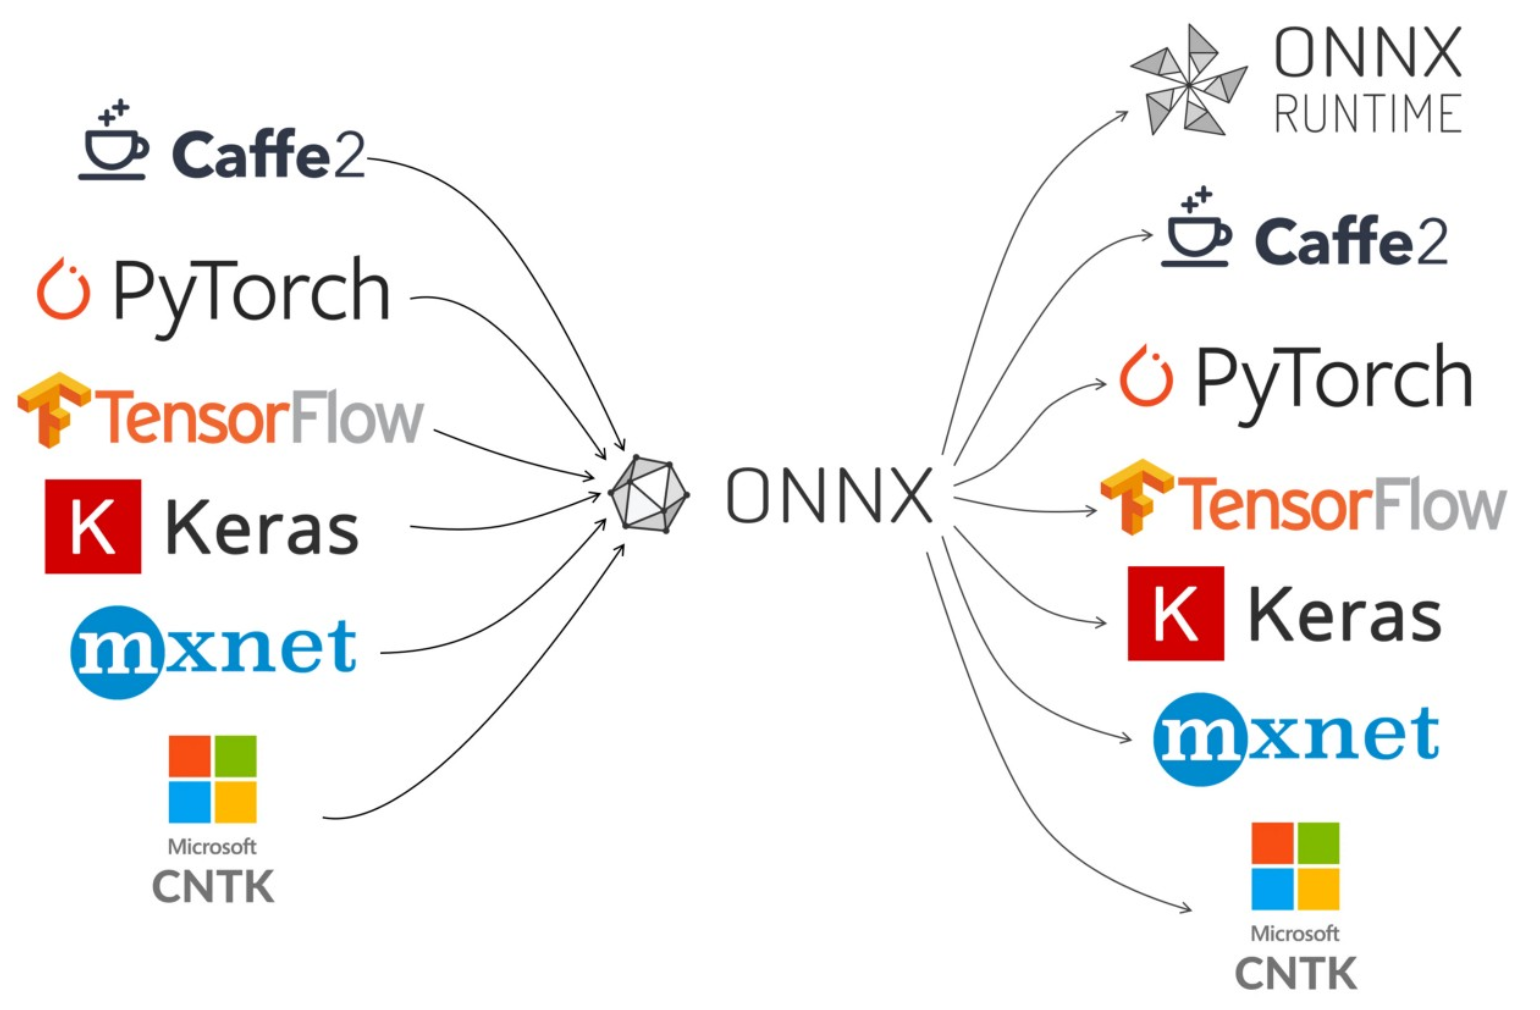
\includegraphics[width=0.7\linewidth]{pics/2-6onnx.png}
  \caption{ONNX 模型转换流程\cite{bai2017onnx}}
  \label{fig:2-6onnx}
\end{figure}

在模型标准化基础上,高效的推理框架成为实现生产部署的核心组件。TensorFlow Serving\cite{olston2017tensorflow} 和 Torch Serve\cite{pytorch2020serve} 是两种广泛使用的推理框架,分别由 TensorFlow 和 PyTorch 社区维护。这些框架通过提供标准化的服务接口和灵活的部署选项,显著降低了模型从开发到生产环境的迁移成本。TensorFlow Serving 基于 gRPC 和 RESTful API 提供高性能的推理服务,其核心设计目标是支持动态模型更新和多版本管理。这使得在分布式环境中运行的推理服务能够实时响应模型更新需求,而无需中断现有服务。此外,TensorFlow Serving 还集成了多种优化技术(如批处理、缓存和硬件加速),从而在保证高吞吐量的同时降低延迟。相比之下,Torch Serve 更加注重易用性和扩展性。它提供了开箱即用的 RESTful API 和自定义处理管道的支持,允许开发者根据具体需求定制推理逻辑。Torch Serve 的模块化架构使其能够轻松集成到现有的 DevOps 流程中,并通过容器化技术(如 Docker 和 Kubernetes)实现高效的服务编排与资源调度。

\section{Actor 编程模式}

\subsection{Actor 编程模型}

Actor 模型是一种通用的并发计算模式,由一组相互隔离且并发运行的 Actor 构成,这些 Actor 通过透明的消息传递机制进行交互 \cite{agha1986actors}。在该模型中,基本计算单元是 Actor,它是一个能够通过网络消息与其他 Actor 进行通信的独立实体 \cite{hewitt2010actor}。Actor 模型继承了面向对象语言的核心思想,并进一步分离了业务逻辑与控制流,从而提升了系统的模块化程度和可维护性。同时,Actor 模型支持将复杂系统分解为多个独立、自主且相互协作的组件,显著简化了开发过程并提高了并行处理效率 \cite{srirama2021akka}。

在分布式环境中,Actor 的设计天然避免了传统并发模型中的资源争用问题。每个 Actor 拥有独立的状态,其状态只能通过接收到的消息进行更新,这种机制确保了 Actor 之间不会相互干扰,从而有效防止了竞态条件的发生。为了应对复杂的任务负载,Actor 模型引入了动态任务分配机制:当某个 Actor 接收到任务时,可以通过 \texttt{spawn} 操作在网络中动态创建新的 Actor 实例,从而实现工作负载的分而治之。例如,在物联网(IoT)应用程序中,传入的任务通常被划分为多个子任务,并通过 \texttt{spawn} 操作分配给新创建的 Actor 进行并发处理,这不仅加快了任务执行速度,还显著缩短了系统的响应时间。此外,每个 Actor 在任务处理过程中会持续监控网络中其他 Actor 的状态,以便及时检测错误并传播相关信息,从而增强了系统的容错能力,使分布式环境中的错误能够被快速定位和处理。

\begin{figure}[ht]
  \centering
  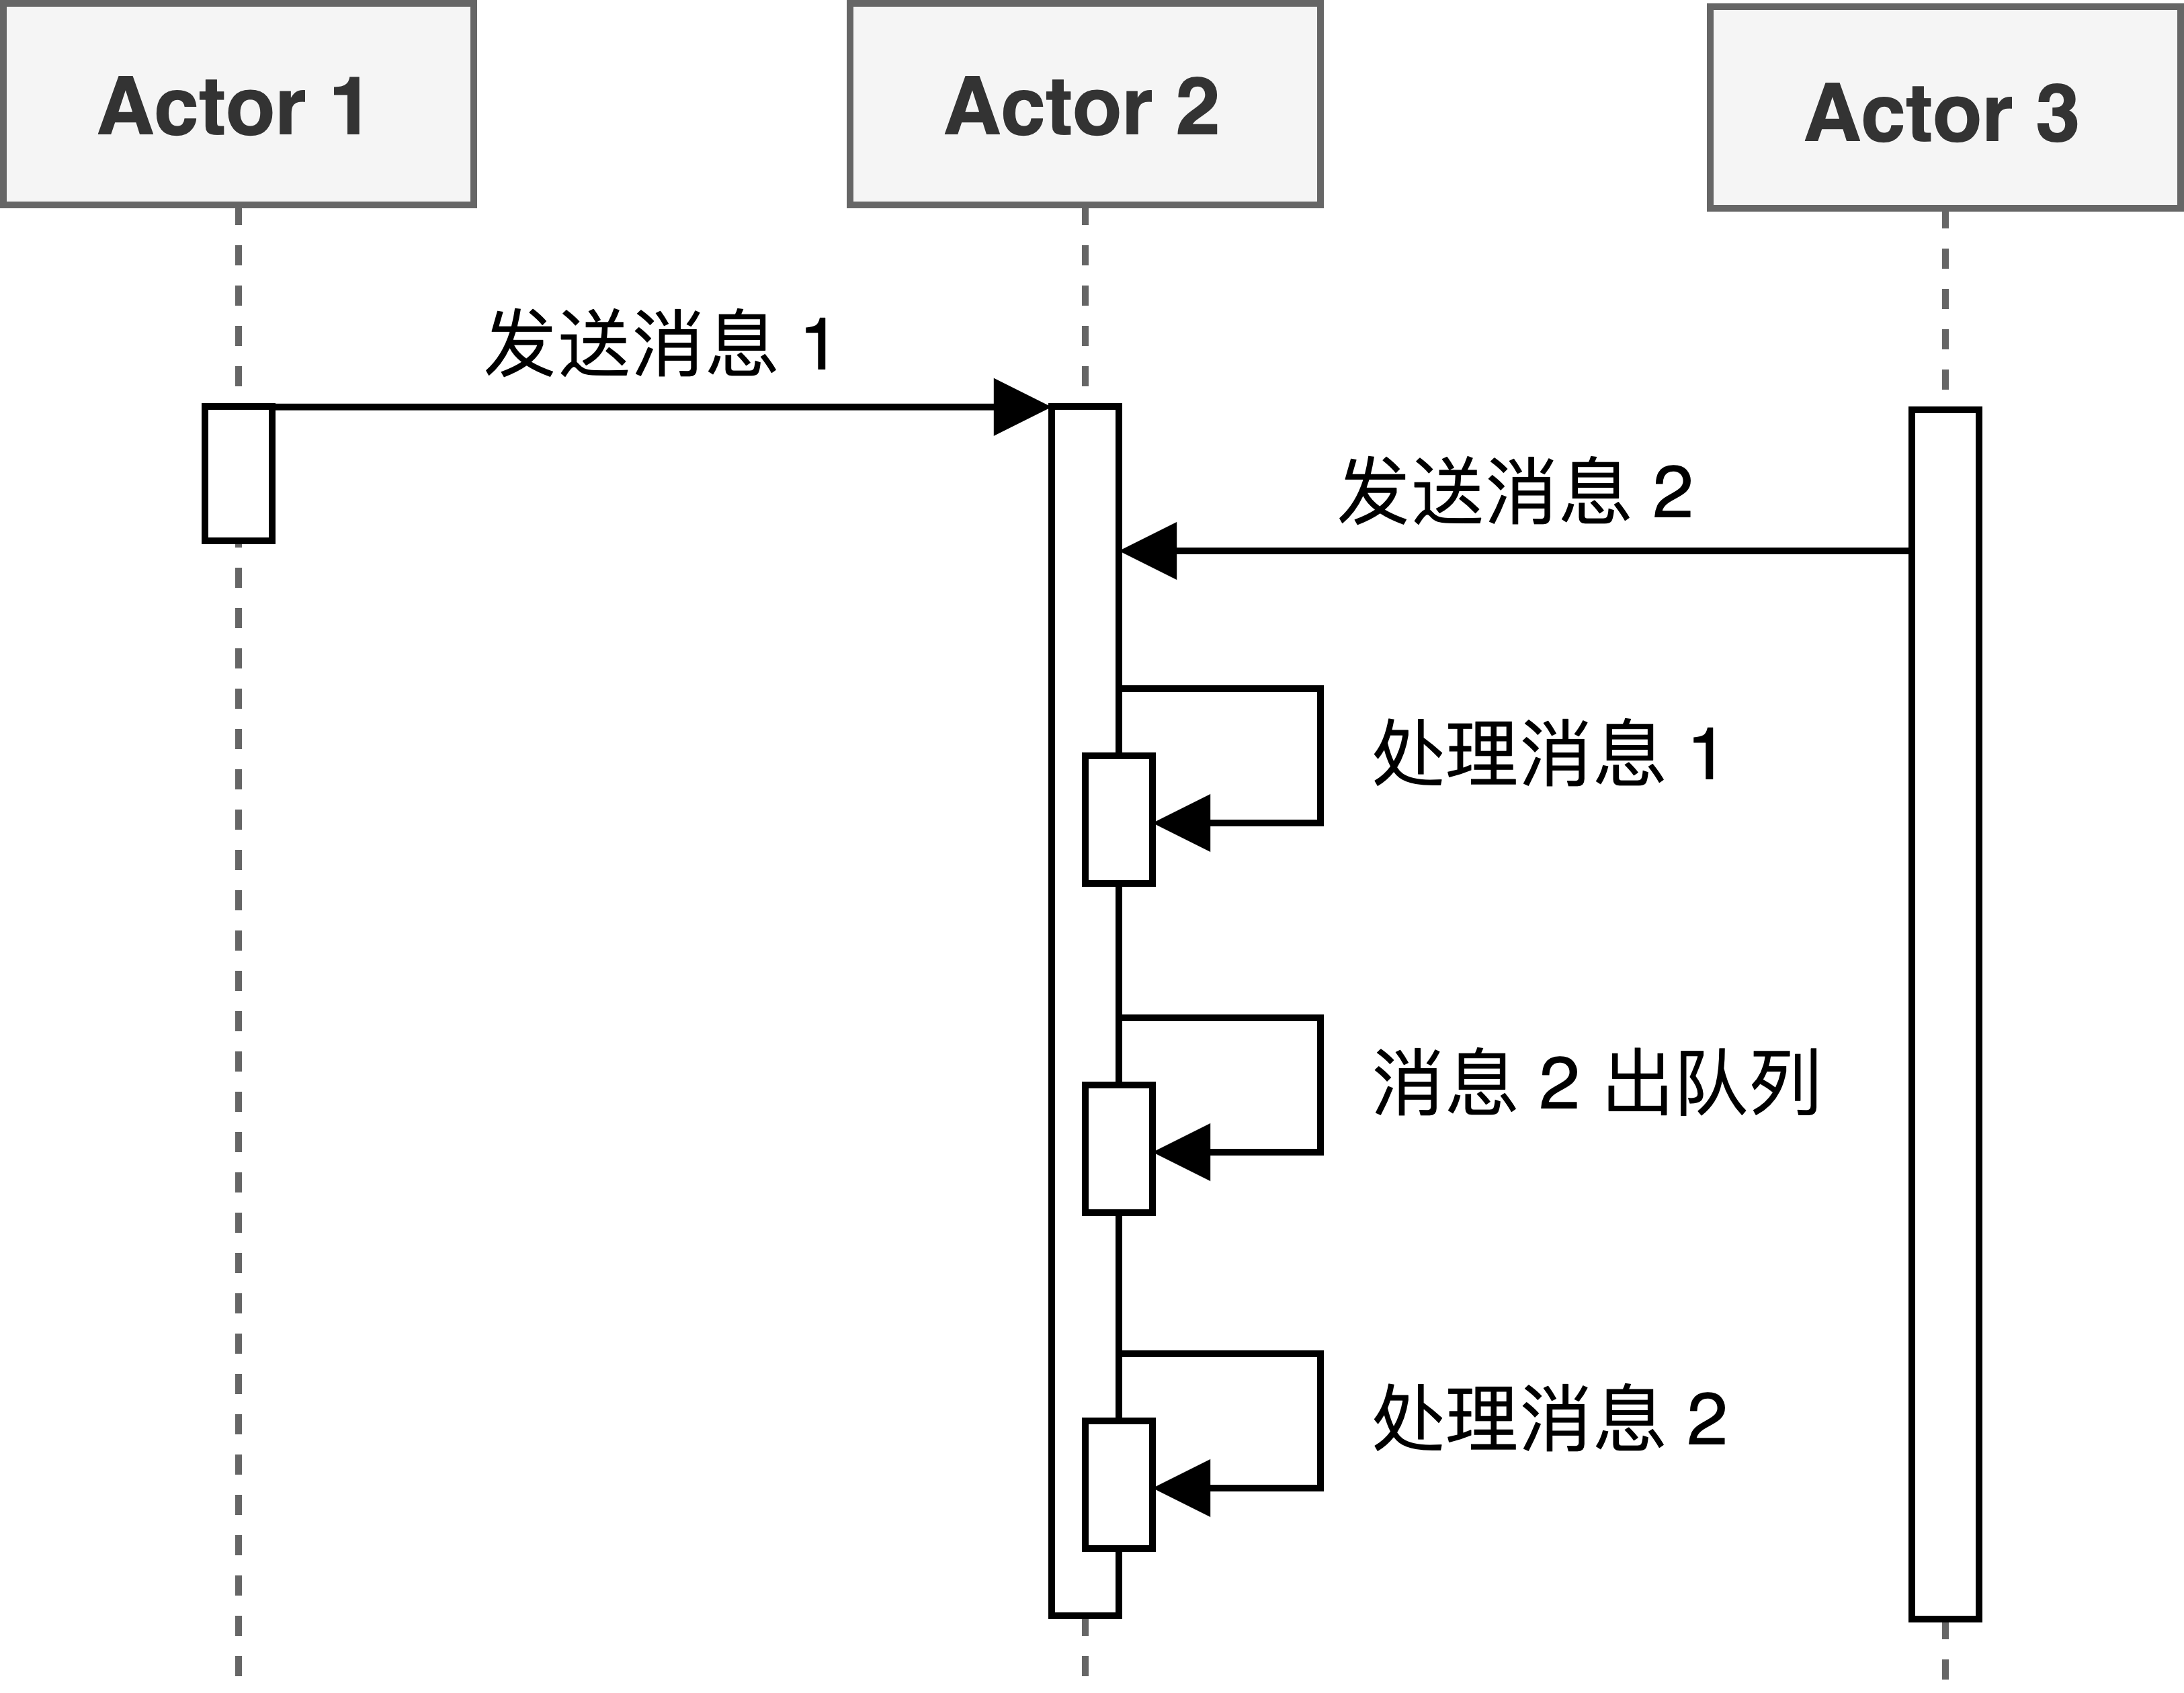
\includegraphics[width=0.65\linewidth]{pics/2-7actormodel.png}
  \caption{多Actor的消息传递和处理流程的时序图\cite{srirama2021akka}}
  \label{fig:2-7actormodel}
\end{figure} 

从实现角度来看,Actor 具有状态和行为,类似于面向对象编程中的对象,但具有更严格的限制。Actor 的状态完全由其自身拥有,不能被系统中的其他 Actor 共享或访问,因此在多线程环境中无需锁或其他同步机制。Actor 的行为由其内部变量和状态组成,通过按顺序处理消息来完成计算,如图\ref{fig:2-7actormodel}所示。具体而言,Actor 的处理流程如下:首先,Actor 将当前消息添加到队列末尾;如果 Actor 正忙且未被调度,则标记消息为待处理状态;随后,隐藏的调度器从队列中取出就绪消息并开始处理;Actor 修改其状态并将消息传递给其他 Actor;最后,Actor 从队列中移除已处理的消息。为支持上述流程,Actor 需具备以下特性:一个基于先进先出原则的邮箱用于存储消息;一组包含内部变量和状态的行为定义;传入消息中包含数据及其参数;一个处理环境用于调用 Actor 的消息处理代码;以及一个唯一地址用于标识 Actor 并分配消息。

在实际应用中,Actor 可以通过以下方式响应消息:向其他 Actor 发送消息以分担负载和进一步处理;根据网络需求动态创建新 Actor;或指定自身行为以处理下一条消息。由于每个 Actor 同时最多只处理一条消息,因此无需同步即可保持一致性。这一特性使得 Actor 模型实现了发送消息与处理消息的解耦,支持异步通信。Actor 之间的连接可以基于物理连接、内存/磁盘访问、网络地址或电子邮件地址等,具体地址形式取决于连接类型。消息传递遵循“尽力而为”原则,一旦发送消息,接收方负责处理,这种“即发即忘”的通信方式进一步增强了系统的灵活性和解耦性。

在过去的几十年中,研究者们设计了多种基于 Actor 模型的语言 \cite{agha1990concurrent}。其中,Erlang 由 Armstrong 开发,旨在支持构建高可用性分布式系统\cite{armstrong2007history}。此外,Scala 是另一种支持 Actor 模型的编程语言,其通过 Akka 框架提供了对 Actor 的原生支持。Scala 运行于 Java 虚拟机(JVM)之上,并兼具函数式编程与面向对象编程(OOP)的特性。近年来,随着云计算和边缘计算(Fog Computing)的兴起,Actor 编程模型在分布式系统中的应用得到了显著推动。特别是在边缘计算环境中,可扩展性和容错性成为处理和分析物联网(IoT)应用程序的关键特性 \cite{srirama2021akka}。

\subsection{Akka 工具包}

Akka 是一个基于 Actor 模型的开源工具包和运行时,旨在简化分布式系统的开发。它由 Lightbend 开发并维护,广泛应用于构建高并发、可扩展且容错性强的分布式应用程序。Akka 的设计核心是将复杂的分布式系统抽象为一组独立的 Actor,从而降低了开发者在处理分布式一致性、负载均衡和容错性等问题上的复杂度。通过这种抽象,Akka 使开发者能够专注于业务逻辑。如图 \ref{fig:2-8akka} 所示,Akka 提供了完整的生命周期管理机制,每个阶段均提供了钩子方法(hook),允许开发者通过重写这些方法来定制化 Actor 的行为,而无需过多关注底层的分布式通信和状态管理细节。

\begin{figure}[ht]
  \centering
  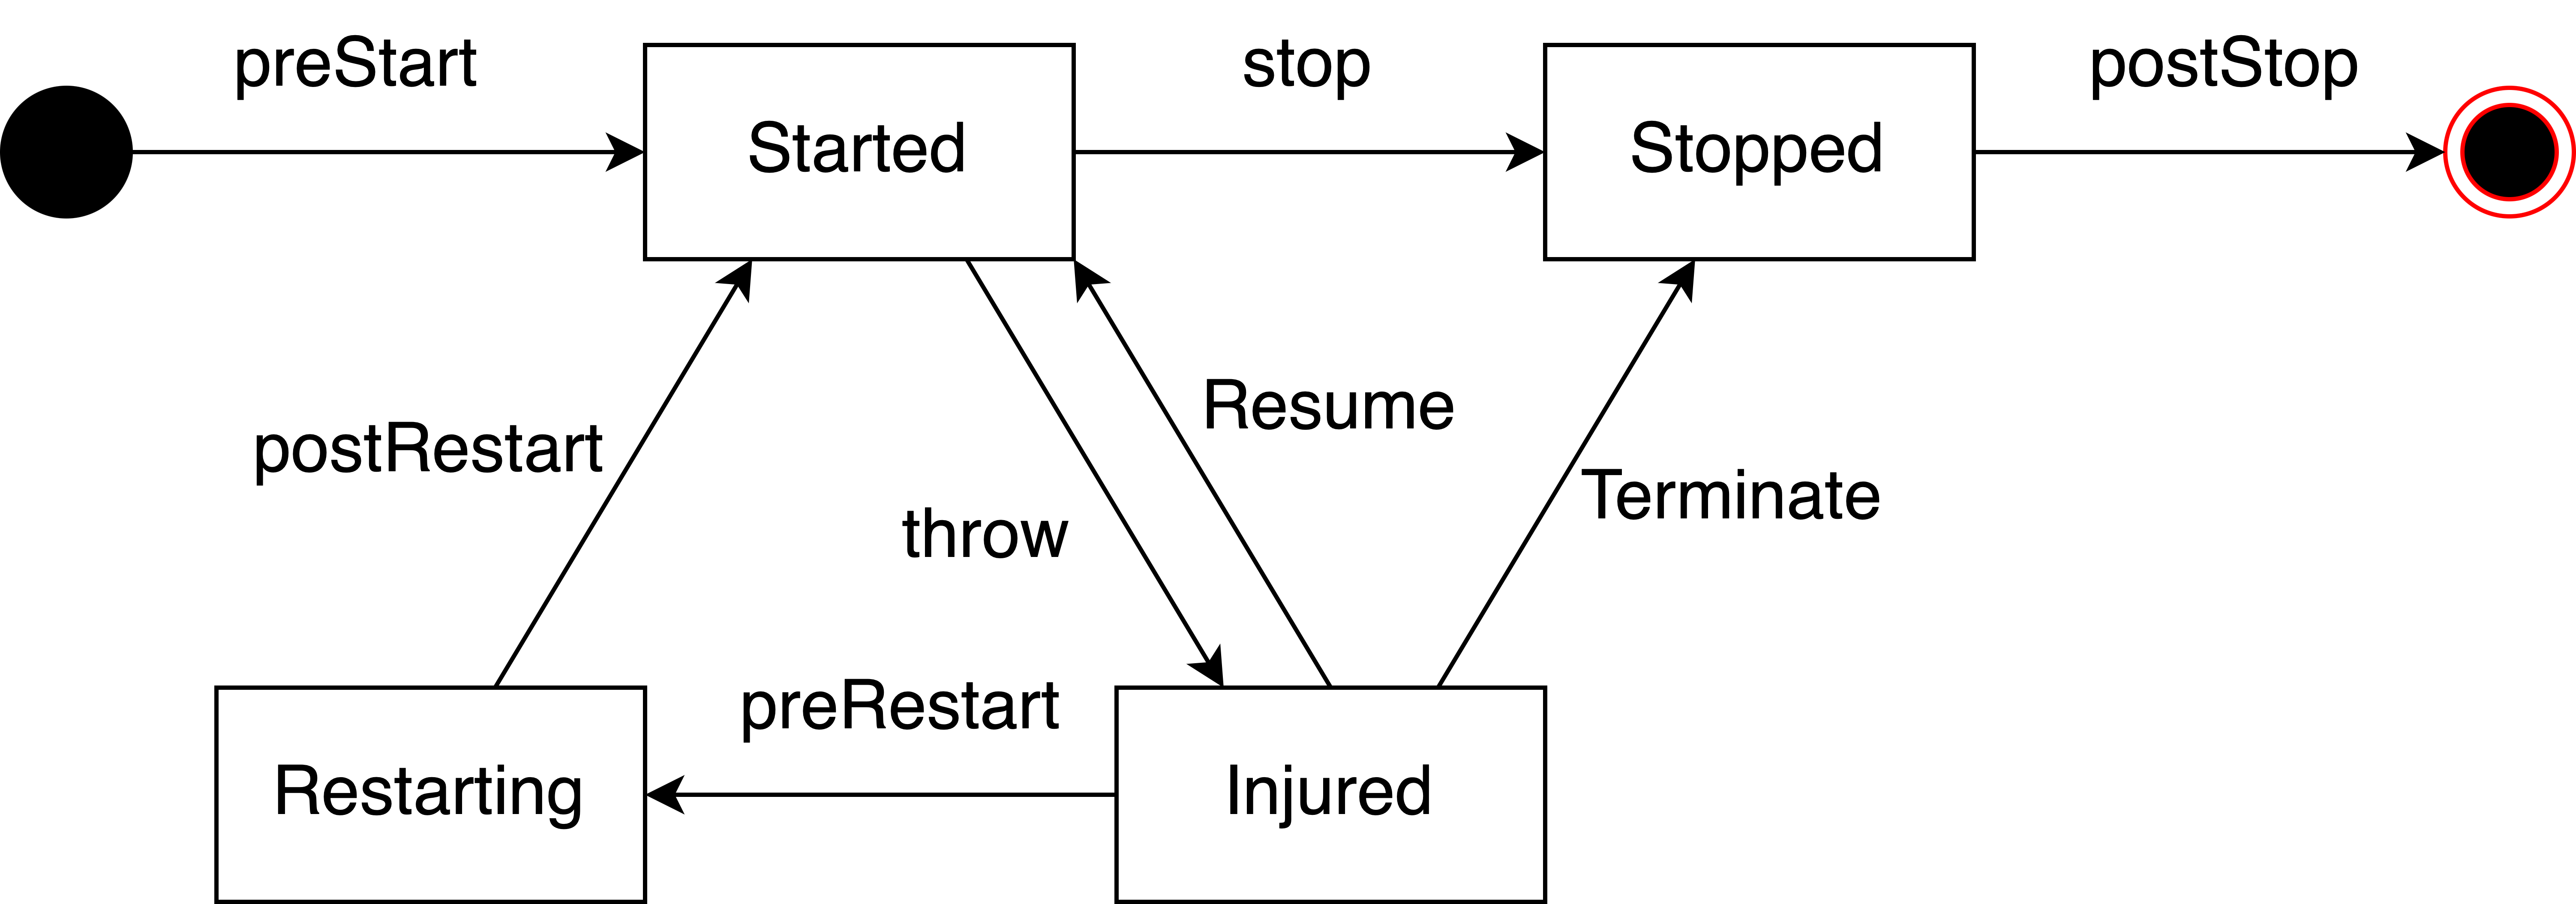
\includegraphics[width=0.8\linewidth]{pics/2-8akka.png}
  \caption{Akka Actor 生命周期}
  \label{fig:2-8akka}
\end{figure} 

Akka 的集群模块(Akka Cluster)和流处理框架(Akka Streams)是其分布式能力的两大核心组件。Akka Cluster 提供了去中心化的集群管理机制,支持节点的动态加入和退出,确保系统在高并发和网络不稳定环境下的弹性扩展与高可用性。它基于 Gossip 协议实现节点间的状态同步,并通过分片(Sharding)机制将任务均匀分布到集群中的不同节点,避免单点过载问题。这种设计特别适合云边协同场景,能够灵活应对边缘设备连接状态和计算能力的动态变化。与此同时,Akka Streams 提供了一种声明式的流处理框架,专注于解决传统流处理中的背压(Backpressure)问题。通过 Reactive Streams 规范,消费者可以动态反馈其处理能力,从而实现流量控制,避免数据生成速度超过消费速度导致的系统崩溃。Akka Streams 还支持复杂的流操作和灵活的拓扑结构设计,使其能够高效处理多源异构数据流,满足边缘计算环境中对实时性和多样性的需求。

\section{本章小结}

本章围绕云边协同、云原生、模型部署以及Actor编程模式的核心内容展开,系统性地介绍了相关技术背景及其应用。首先,从云边协同的基本概念切入,深入剖析了“端-边-云”三层架构的设计理念,并对其在垂直与水平方向上的优化策略进行了详细探讨。其次,聚焦云原生技术体系,依次阐述了容器化技术、Kubernetes集群管理以及系统监控等关键技术,为实现高效的分布式云边协同提供了理论支持和技术保障。在此基础上,进一步探讨了推理部署的关键环节,展示了其在实际应用中的重要性。最后,针对分布式系统的开发需求,引入了基于Actor模型的Akka框架,并对其设计原理和适用场景进行了深入分析,为后续研究奠定了坚实基础。

